\chapter{Технологический раздел}

\section{Выбор языка программирования и среды разработки}

В качестве языка программирования был выбран C\# в силу следующих причин:

\begin{itemize}[label=---]
	\item В стандартной библиотеке языка присутствует поддержка всех структур данных, выбранных по результатам проектирования;
	\item C\# обладает обширной экосистемой библиотек, которые упрощают работу с базой данных PostgreSQL, обеспечивая удобное подключение, выполнение запросов и управление данными.;
\end{itemize}

В качестве среды разработки была выбрана Microsoft Visual Studio 2022 как версия единственной на данный момент среды, полностью поддерживающей последний стандарт языка C\#

\section{Выбор СУБД}

PostgreSQL была выбрана в качестве СУБД \cite{5}:
\begin{itemize}[label=---]
	\item PostgreSQL распространяется с открытым исходным кодом, что означает отсутствие лицензионных затрат и свободу в настройке и расширении системы под нужды конкретного проекта. Это делает её идеальным выбором для стартапов и малых предприятий, а также крупных организаций;
	\item PostgreSQL может работать как с реляционными (структурированными) данными, так и с нереляционными (неструктурированными), такими как JSON, XML и HSTORE. Это делает её идеальной для гибридных систем, требующих универсальности в работе с данными;
	\item Поддерживает основные платформы, включая Linux, Windows и macOS, что делает её универсальной для различных операционных систем;
	\item Встроенные функции безопасности, такие как поддержка DBMS\_SESSION для управления сессиями пользователей, сложные механизмы контроля доступа, а также возможность шифрования данных на уровне транспортного слоя (SSL), делают PostgreSQL надёжным выбором для работы с конфиденциальной информацией;
\end{itemize}

\section{Создание объектов баз данных}
Ниже, на листинге \ref{lst:UserDB} - \ref{lst:DetailBillDB}, представлено создание всех таблиц.

\begin{center}
	\captionsetup{justification=raggedright,singlelinecheck=off}
	\begin{lstlisting}[label=lst:UserDB,caption=Создание таблицы UserDB]
		create table UserDB(
		Id serial primary key,
		Name varchar(50) not null,
		Phone varchar(50) not null,
		Address varchar(50) not null,
		Email varchar(50) not null,
		Login varchar(50) unique,
		Password varchar(50) not null,
		Role varchar(50) not null check (role in ('admin', 'seller', 'client'))
		);
	\end{lstlisting}
\end{center}

\begin{center}
	\captionsetup{justification=raggedright,singlelinecheck=off}
	\begin{lstlisting}[label=lst:CategoryDB, language=sql,caption=Создание таблицы PromoDB]
		create table PromoDB(
		Id serial primary key,
		code varchar(20) unique,
		discount int not null,
		data_start date not null,
		data_end date not null
		);
	\end{lstlisting}
\end{center}

\clearpage
\begin{center}
	\captionsetup{justification=raggedright,singlelinecheck=off}
	\begin{lstlisting}[label=lst:PublisherDB, language=sql,caption=Создание таблицы ProductDB]
		create table ProductDB (
		Id serial primary key,
		Name varchar(50) not null,
		Price int not null,
		Quantity int not null,
		Manufacturer varchar(50) not null,
		Description varchar(50) not null
		);
	\end{lstlisting}
\end{center}

\begin{center}
	\captionsetup{justification=raggedright,singlelinecheck=off}
	\begin{lstlisting}[label=lst:AuthorDB, language=sql,caption=Создание таблицы CartDB]
		create table CartDB(
		Id serial primary key,
		data_created date not null,
		id_user int references UserDB(Id) ON DELETE CASCADE
		);
	\end{lstlisting}
\end{center}

\begin{center}
	\captionsetup{justification=raggedright,singlelinecheck=off}
	\begin{lstlisting}[label=lst:ItemDB, language=sql,caption=Создание таблицы ItemCartDB]
		create table ItemCartDB(
		Id serial primary key,
		id_product int,
		id_cart int,
		quantity int not null,
		foreign key (id_cart) references CartDB(Id) ON DELETE CASCADE,
		foreign key (id_product) references ProductDB(Id) ON DELETE CASCADE
		);
	\end{lstlisting}
\end{center}

\begin{center}
	\captionsetup{justification=raggedright,singlelinecheck=off}
	\begin{lstlisting}[label=lst:BillDB, language=sql,caption=Создание таблицы OrderDB]
		create table orderDB(
		Id serial primary key,
		status varchar(20) not null,
		data_created date not null,
		id_user int not null,
		id_promo int references PromoDB(Id) ON DELETE CASCADE,
		foreign key (id_user) references UserDB(Id) ON DELETE CASCADE
		);
		
	\end{lstlisting}
\end{center}

\begin{center}
	\captionsetup{justification=raggedright,singlelinecheck=off}
	\begin{lstlisting}[label=lst:DetailBillDB, language=sql,caption=Создание таблицы ItemOrderDB]
		create table ItemOrderDB(
		Id serial primary key,
		id_product int not null,
		id_order int not null,
		quantity int  not null,
		foreign key (id_order) references OrderDB(Id) ON DELETE CASCADE,
		foreign key (id_product) references ProductDB(Id) ON DELETE CASCADE
		);
	\end{lstlisting}
\end{center}

\section{Реализация программы}
На листингах \ref{lst:pro1} - \ref{lst:pro2} в приложении A представлены примеры основных функций программы, реализующие ключевые действия пользователей, такие как редактирование товаров и редактирование информации о пользователях. Эти функции включают в себя обработку пользовательских данных, валидацию ввода и взаимодействие с базой данных для обновления соответствующих записей. Примеры кода демонстрируют архитектуру приложения и логику выполнения операций по управлению товарами и пользовательскими данными.

\section{Интерфейс программы}

На рисунках \ref{img:ex1} -- \ref{img:ex10} в приложении A отображён интерфейс приложения. Эти изображения соответствуют каждой роли пользователя и их операции.
Каждый рисунок иллюстрирует различные экраны и элементы интерфейса, соответствующие операциям, которые могут выполнять пользователи в зависимости от их роли.

Для каждой роли пользователя предусмотрены свои функции и права доступа. Интерфейс адаптирован под разные задачи, такие как редактирование товаров, управление учетными записями пользователей, просмотр и изменение данных, а также выполнение административных операций.

Изображения демонстрируют ключевые элементы взаимодействия, включая формы для ввода и редактирования данных, элементы навигации, кнопки действий, а также сообщения об успешных операциях или ошибках. Весь интерфейс разработан с учётом требований удобства и простоты использования, что делает приложение доступным для пользователей с любым уровнем технической подготовки. Кроме того, все операции сопровождаются соответствующей валидацией и обработкой ошибок, что повышает стабильность работы приложения и защищает его от некорректного ввода данных.

\section{Тестирование триггера}
На листинге \ref{lst:trigger} в приложении A представлено создание триггера, который автоматически рассчитывает количество товаров на складе когда клиент размещает заказ.

Проводится тестирование триггера, который автоматически обновляет значение поля quantity в таблице productdb, отражающее количество доступных товаров на складе. Триггер срабатывает каждый раз, когда клиент совершает заказ, уменьшает количество товаров на складе в соответствии с числом заказанных единиц, и записывает обновлённое значение в базу данных.

Тестирование включает в себя проверку корректности работы триггера в различных сценариях. Важно убедиться, что триггер правильно уменьшает quantity только после успешного оформления заказа и что нет расхождений между фактическим и заявленным количеством товаров.

На листинге \ref{lst:test2} в приложении A представлена функция тестирования триггера.

На рисунке \ref{img:test} представлена функция, предназначенная для тестирования триггера, который обновляет количество товаров на складе.
\begin{figure}[ht!]
	\centering
	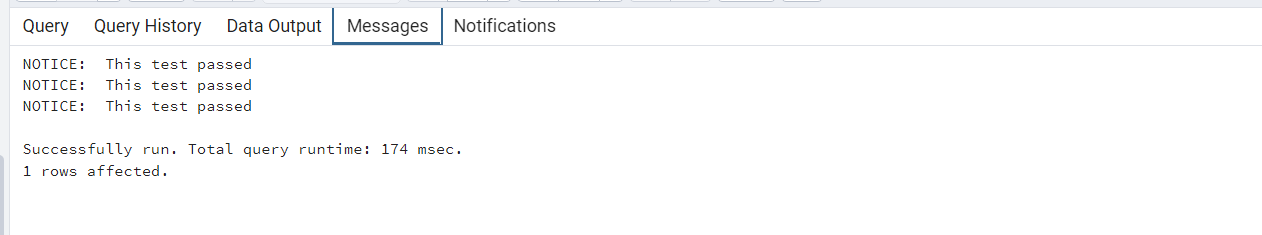
\includegraphics[width=0.8\linewidth]{img/test.png}
	\caption{Результаты тестов для триггера after\_itemorder\_insert.}
	\label{img:test}
\end{figure}

\subsection*{Вывод}
В данном разделе представлены средства разработки программного обеспечения, выбор языка программирования и описан интерфейс программы. Также рассмотрены примеры работы программы.